\documentclass[10pt]{article}
\usepackage{tmlr}
% Camera-ready only:
%\usepackage[accepted]{tmlr}
% To de-anonymize for a preprint:
%\usepackage[preprint]{tmlr}

%%%%% NEW MATH DEFINITIONS %%%%%

\usepackage{amsmath,amsfonts,bm}

% Mark sections of captions for referring to divisions of figures
\newcommand{\figleft}{{\em (Left)}}
\newcommand{\figcenter}{{\em (Center)}}
\newcommand{\figright}{{\em (Right)}}
\newcommand{\figtop}{{\em (Top)}}
\newcommand{\figbottom}{{\em (Bottom)}}
\newcommand{\captiona}{{\em (a)}}
\newcommand{\captionb}{{\em (b)}}
\newcommand{\captionc}{{\em (c)}}
\newcommand{\captiond}{{\em (d)}}

% Highlight a newly defined term
\newcommand{\newterm}[1]{{\bf #1}}


% Figure reference, lower-case.
\def\figref#1{figure~\ref{#1}}
% Figure reference, capital. For start of sentence
\def\Figref#1{Figure~\ref{#1}}
\def\twofigref#1#2{figures \ref{#1} and \ref{#2}}
\def\quadfigref#1#2#3#4{figures \ref{#1}, \ref{#2}, \ref{#3} and \ref{#4}}
% Section reference, lower-case.
\def\secref#1{section~\ref{#1}}
% Section reference, capital.
\def\Secref#1{Section~\ref{#1}}
% Reference to two sections.
\def\twosecrefs#1#2{sections \ref{#1} and \ref{#2}}
% Reference to three sections.
\def\secrefs#1#2#3{sections \ref{#1}, \ref{#2} and \ref{#3}}
% Reference to an equation, lower-case.
\def\eqref#1{equation~\ref{#1}}
% Reference to an equation, upper case
\def\Eqref#1{Equation~\ref{#1}}
% A raw reference to an equation---avoid using if possible
\def\plaineqref#1{\ref{#1}}
% Reference to a chapter, lower-case.
\def\chapref#1{chapter~\ref{#1}}
% Reference to an equation, upper case.
\def\Chapref#1{Chapter~\ref{#1}}
% Reference to a range of chapters
\def\rangechapref#1#2{chapters\ref{#1}--\ref{#2}}
% Reference to an algorithm, lower-case.
\def\algref#1{algorithm~\ref{#1}}
% Reference to an algorithm, upper case.
\def\Algref#1{Algorithm~\ref{#1}}
\def\twoalgref#1#2{algorithms \ref{#1} and \ref{#2}}
\def\Twoalgref#1#2{Algorithms \ref{#1} and \ref{#2}}
% Reference to a part, lower case
\def\partref#1{part~\ref{#1}}
% Reference to a part, upper case
\def\Partref#1{Part~\ref{#1}}
\def\twopartref#1#2{parts \ref{#1} and \ref{#2}}

\def\ceil#1{\lceil #1 \rceil}
\def\floor#1{\lfloor #1 \rfloor}
\def\1{\bm{1}}
\newcommand{\train}{\mathcal{D}}
\newcommand{\valid}{\mathcal{D_{\mathrm{valid}}}}
\newcommand{\test}{\mathcal{D_{\mathrm{test}}}}

\def\eps{{\epsilon}}


% Random variables
\def\reta{{\textnormal{$\eta$}}}
\def\ra{{\textnormal{a}}}
\def\rb{{\textnormal{b}}}
\def\rc{{\textnormal{c}}}
\def\rd{{\textnormal{d}}}
\def\re{{\textnormal{e}}}
\def\rf{{\textnormal{f}}}
\def\rg{{\textnormal{g}}}
\def\rh{{\textnormal{h}}}
\def\ri{{\textnormal{i}}}
\def\rj{{\textnormal{j}}}
\def\rk{{\textnormal{k}}}
\def\rl{{\textnormal{l}}}
% rm is already a command, just don't name any random variables m
\def\rn{{\textnormal{n}}}
\def\ro{{\textnormal{o}}}
\def\rp{{\textnormal{p}}}
\def\rq{{\textnormal{q}}}
\def\rr{{\textnormal{r}}}
\def\rs{{\textnormal{s}}}
\def\rt{{\textnormal{t}}}
\def\ru{{\textnormal{u}}}
\def\rv{{\textnormal{v}}}
\def\rw{{\textnormal{w}}}
\def\rx{{\textnormal{x}}}
\def\ry{{\textnormal{y}}}
\def\rz{{\textnormal{z}}}

% Random vectors
\def\rvepsilon{{\mathbf{\epsilon}}}
\def\rvtheta{{\mathbf{\theta}}}
\def\rva{{\mathbf{a}}}
\def\rvb{{\mathbf{b}}}
\def\rvc{{\mathbf{c}}}
\def\rvd{{\mathbf{d}}}
\def\rve{{\mathbf{e}}}
\def\rvf{{\mathbf{f}}}
\def\rvg{{\mathbf{g}}}
\def\rvh{{\mathbf{h}}}
\def\rvu{{\mathbf{i}}}
\def\rvj{{\mathbf{j}}}
\def\rvk{{\mathbf{k}}}
\def\rvl{{\mathbf{l}}}
\def\rvm{{\mathbf{m}}}
\def\rvn{{\mathbf{n}}}
\def\rvo{{\mathbf{o}}}
\def\rvp{{\mathbf{p}}}
\def\rvq{{\mathbf{q}}}
\def\rvr{{\mathbf{r}}}
\def\rvs{{\mathbf{s}}}
\def\rvt{{\mathbf{t}}}
\def\rvu{{\mathbf{u}}}
\def\rvv{{\mathbf{v}}}
\def\rvw{{\mathbf{w}}}
\def\rvx{{\mathbf{x}}}
\def\rvy{{\mathbf{y}}}
\def\rvz{{\mathbf{z}}}

% Elements of random vectors
\def\erva{{\textnormal{a}}}
\def\ervb{{\textnormal{b}}}
\def\ervc{{\textnormal{c}}}
\def\ervd{{\textnormal{d}}}
\def\erve{{\textnormal{e}}}
\def\ervf{{\textnormal{f}}}
\def\ervg{{\textnormal{g}}}
\def\ervh{{\textnormal{h}}}
\def\ervi{{\textnormal{i}}}
\def\ervj{{\textnormal{j}}}
\def\ervk{{\textnormal{k}}}
\def\ervl{{\textnormal{l}}}
\def\ervm{{\textnormal{m}}}
\def\ervn{{\textnormal{n}}}
\def\ervo{{\textnormal{o}}}
\def\ervp{{\textnormal{p}}}
\def\ervq{{\textnormal{q}}}
\def\ervr{{\textnormal{r}}}
\def\ervs{{\textnormal{s}}}
\def\ervt{{\textnormal{t}}}
\def\ervu{{\textnormal{u}}}
\def\ervv{{\textnormal{v}}}
\def\ervw{{\textnormal{w}}}
\def\ervx{{\textnormal{x}}}
\def\ervy{{\textnormal{y}}}
\def\ervz{{\textnormal{z}}}

% Random matrices
\def\rmA{{\mathbf{A}}}
\def\rmB{{\mathbf{B}}}
\def\rmC{{\mathbf{C}}}
\def\rmD{{\mathbf{D}}}
\def\rmE{{\mathbf{E}}}
\def\rmF{{\mathbf{F}}}
\def\rmG{{\mathbf{G}}}
\def\rmH{{\mathbf{H}}}
\def\rmI{{\mathbf{I}}}
\def\rmJ{{\mathbf{J}}}
\def\rmK{{\mathbf{K}}}
\def\rmL{{\mathbf{L}}}
\def\rmM{{\mathbf{M}}}
\def\rmN{{\mathbf{N}}}
\def\rmO{{\mathbf{O}}}
\def\rmP{{\mathbf{P}}}
\def\rmQ{{\mathbf{Q}}}
\def\rmR{{\mathbf{R}}}
\def\rmS{{\mathbf{S}}}
\def\rmT{{\mathbf{T}}}
\def\rmU{{\mathbf{U}}}
\def\rmV{{\mathbf{V}}}
\def\rmW{{\mathbf{W}}}
\def\rmX{{\mathbf{X}}}
\def\rmY{{\mathbf{Y}}}
\def\rmZ{{\mathbf{Z}}}

% Elements of random matrices
\def\ermA{{\textnormal{A}}}
\def\ermB{{\textnormal{B}}}
\def\ermC{{\textnormal{C}}}
\def\ermD{{\textnormal{D}}}
\def\ermE{{\textnormal{E}}}
\def\ermF{{\textnormal{F}}}
\def\ermG{{\textnormal{G}}}
\def\ermH{{\textnormal{H}}}
\def\ermI{{\textnormal{I}}}
\def\ermJ{{\textnormal{J}}}
\def\ermK{{\textnormal{K}}}
\def\ermL{{\textnormal{L}}}
\def\ermM{{\textnormal{M}}}
\def\ermN{{\textnormal{N}}}
\def\ermO{{\textnormal{O}}}
\def\ermP{{\textnormal{P}}}
\def\ermQ{{\textnormal{Q}}}
\def\ermR{{\textnormal{R}}}
\def\ermS{{\textnormal{S}}}
\def\ermT{{\textnormal{T}}}
\def\ermU{{\textnormal{U}}}
\def\ermV{{\textnormal{V}}}
\def\ermW{{\textnormal{W}}}
\def\ermX{{\textnormal{X}}}
\def\ermY{{\textnormal{Y}}}
\def\ermZ{{\textnormal{Z}}}

% Vectors
\def\vzero{{\bm{0}}}
\def\vone{{\bm{1}}}
\def\vmu{{\bm{\mu}}}
\def\vtheta{{\bm{\theta}}}
\def\va{{\bm{a}}}
\def\vb{{\bm{b}}}
\def\vc{{\bm{c}}}
\def\vd{{\bm{d}}}
\def\ve{{\bm{e}}}
\def\vf{{\bm{f}}}
\def\vg{{\bm{g}}}
\def\vh{{\bm{h}}}
\def\vi{{\bm{i}}}
\def\vj{{\bm{j}}}
\def\vk{{\bm{k}}}
\def\vl{{\bm{l}}}
\def\vm{{\bm{m}}}
\def\vn{{\bm{n}}}
\def\vo{{\bm{o}}}
\def\vp{{\bm{p}}}
\def\vq{{\bm{q}}}
\def\vr{{\bm{r}}}
\def\vs{{\bm{s}}}
\def\vt{{\bm{t}}}
\def\vu{{\bm{u}}}
\def\vv{{\bm{v}}}
\def\vw{{\bm{w}}}
\def\vx{{\bm{x}}}
\def\vy{{\bm{y}}}
\def\vz{{\bm{z}}}

% Elements of vectors
\def\evalpha{{\alpha}}
\def\evbeta{{\beta}}
\def\evepsilon{{\epsilon}}
\def\evlambda{{\lambda}}
\def\evomega{{\omega}}
\def\evmu{{\mu}}
\def\evpsi{{\psi}}
\def\evsigma{{\sigma}}
\def\evtheta{{\theta}}
\def\eva{{a}}
\def\evb{{b}}
\def\evc{{c}}
\def\evd{{d}}
\def\eve{{e}}
\def\evf{{f}}
\def\evg{{g}}
\def\evh{{h}}
\def\evi{{i}}
\def\evj{{j}}
\def\evk{{k}}
\def\evl{{l}}
\def\evm{{m}}
\def\evn{{n}}
\def\evo{{o}}
\def\evp{{p}}
\def\evq{{q}}
\def\evr{{r}}
\def\evs{{s}}
\def\evt{{t}}
\def\evu{{u}}
\def\evv{{v}}
\def\evw{{w}}
\def\evx{{x}}
\def\evy{{y}}
\def\evz{{z}}

% Matrix
\def\mA{{\bm{A}}}
\def\mB{{\bm{B}}}
\def\mC{{\bm{C}}}
\def\mD{{\bm{D}}}
\def\mE{{\bm{E}}}
\def\mF{{\bm{F}}}
\def\mG{{\bm{G}}}
\def\mH{{\bm{H}}}
\def\mI{{\bm{I}}}
\def\mJ{{\bm{J}}}
\def\mK{{\bm{K}}}
\def\mL{{\bm{L}}}
\def\mM{{\bm{M}}}
\def\mN{{\bm{N}}}
\def\mO{{\bm{O}}}
\def\mP{{\bm{P}}}
\def\mQ{{\bm{Q}}}
\def\mR{{\bm{R}}}
\def\mS{{\bm{S}}}
\def\mT{{\bm{T}}}
\def\mU{{\bm{U}}}
\def\mV{{\bm{V}}}
\def\mW{{\bm{W}}}
\def\mX{{\bm{X}}}
\def\mY{{\bm{Y}}}
\def\mZ{{\bm{Z}}}
\def\mBeta{{\bm{\beta}}}
\def\mPhi{{\bm{\Phi}}}
\def\mLambda{{\bm{\Lambda}}}
\def\mSigma{{\bm{\Sigma}}}

% Tensor
\DeclareMathAlphabet{\mathsfit}{\encodingdefault}{\sfdefault}{m}{sl}
\SetMathAlphabet{\mathsfit}{bold}{\encodingdefault}{\sfdefault}{bx}{n}
\newcommand{\tens}[1]{\bm{\mathsfit{#1}}}
\def\tA{{\tens{A}}}
\def\tB{{\tens{B}}}
\def\tC{{\tens{C}}}
\def\tD{{\tens{D}}}
\def\tE{{\tens{E}}}
\def\tF{{\tens{F}}}
\def\tG{{\tens{G}}}
\def\tH{{\tens{H}}}
\def\tI{{\tens{I}}}
\def\tJ{{\tens{J}}}
\def\tK{{\tens{K}}}
\def\tL{{\tens{L}}}
\def\tM{{\tens{M}}}
\def\tN{{\tens{N}}}
\def\tO{{\tens{O}}}
\def\tP{{\tens{P}}}
\def\tQ{{\tens{Q}}}
\def\tR{{\tens{R}}}
\def\tS{{\tens{S}}}
\def\tT{{\tens{T}}}
\def\tU{{\tens{U}}}
\def\tV{{\tens{V}}}
\def\tW{{\tens{W}}}
\def\tX{{\tens{X}}}
\def\tY{{\tens{Y}}}
\def\tZ{{\tens{Z}}}


% Graph
\def\gA{{\mathcal{A}}}
\def\gB{{\mathcal{B}}}
\def\gC{{\mathcal{C}}}
\def\gD{{\mathcal{D}}}
\def\gE{{\mathcal{E}}}
\def\gF{{\mathcal{F}}}
\def\gG{{\mathcal{G}}}
\def\gH{{\mathcal{H}}}
\def\gI{{\mathcal{I}}}
\def\gJ{{\mathcal{J}}}
\def\gK{{\mathcal{K}}}
\def\gL{{\mathcal{L}}}
\def\gM{{\mathcal{M}}}
\def\gN{{\mathcal{N}}}
\def\gO{{\mathcal{O}}}
\def\gP{{\mathcal{P}}}
\def\gQ{{\mathcal{Q}}}
\def\gR{{\mathcal{R}}}
\def\gS{{\mathcal{S}}}
\def\gT{{\mathcal{T}}}
\def\gU{{\mathcal{U}}}
\def\gV{{\mathcal{V}}}
\def\gW{{\mathcal{W}}}
\def\gX{{\mathcal{X}}}
\def\gY{{\mathcal{Y}}}
\def\gZ{{\mathcal{Z}}}

% Sets
\def\sA{{\mathbb{A}}}
\def\sB{{\mathbb{B}}}
\def\sC{{\mathbb{C}}}
\def\sD{{\mathbb{D}}}
% Don't use a set called E, because this would be the same as our symbol
% for expectation.
\def\sF{{\mathbb{F}}}
\def\sG{{\mathbb{G}}}
\def\sH{{\mathbb{H}}}
\def\sI{{\mathbb{I}}}
\def\sJ{{\mathbb{J}}}
\def\sK{{\mathbb{K}}}
\def\sL{{\mathbb{L}}}
\def\sM{{\mathbb{M}}}
\def\sN{{\mathbb{N}}}
\def\sO{{\mathbb{O}}}
\def\sP{{\mathbb{P}}}
\def\sQ{{\mathbb{Q}}}
\def\sR{{\mathbb{R}}}
\def\sS{{\mathbb{S}}}
\def\sT{{\mathbb{T}}}
\def\sU{{\mathbb{U}}}
\def\sV{{\mathbb{V}}}
\def\sW{{\mathbb{W}}}
\def\sX{{\mathbb{X}}}
\def\sY{{\mathbb{Y}}}
\def\sZ{{\mathbb{Z}}}

% Entries of a matrix
\def\emLambda{{\Lambda}}
\def\emA{{A}}
\def\emB{{B}}
\def\emC{{C}}
\def\emD{{D}}
\def\emE{{E}}
\def\emF{{F}}
\def\emG{{G}}
\def\emH{{H}}
\def\emI{{I}}
\def\emJ{{J}}
\def\emK{{K}}
\def\emL{{L}}
\def\emM{{M}}
\def\emN{{N}}
\def\emO{{O}}
\def\emP{{P}}
\def\emQ{{Q}}
\def\emR{{R}}
\def\emS{{S}}
\def\emT{{T}}
\def\emU{{U}}
\def\emV{{V}}
\def\emW{{W}}
\def\emX{{X}}
\def\emY{{Y}}
\def\emZ{{Z}}
\def\emSigma{{\Sigma}}

% entries of a tensor
% Same font as tensor, without \bm wrapper
\newcommand{\etens}[1]{\mathsfit{#1}}
\def\etLambda{{\etens{\Lambda}}}
\def\etA{{\etens{A}}}
\def\etB{{\etens{B}}}
\def\etC{{\etens{C}}}
\def\etD{{\etens{D}}}
\def\etE{{\etens{E}}}
\def\etF{{\etens{F}}}
\def\etG{{\etens{G}}}
\def\etH{{\etens{H}}}
\def\etI{{\etens{I}}}
\def\etJ{{\etens{J}}}
\def\etK{{\etens{K}}}
\def\etL{{\etens{L}}}
\def\etM{{\etens{M}}}
\def\etN{{\etens{N}}}
\def\etO{{\etens{O}}}
\def\etP{{\etens{P}}}
\def\etQ{{\etens{Q}}}
\def\etR{{\etens{R}}}
\def\etS{{\etens{S}}}
\def\etT{{\etens{T}}}
\def\etU{{\etens{U}}}
\def\etV{{\etens{V}}}
\def\etW{{\etens{W}}}
\def\etX{{\etens{X}}}
\def\etY{{\etens{Y}}}
\def\etZ{{\etens{Z}}}

% The true underlying data generating distribution
\newcommand{\pdata}{p_{\rm{data}}}
% The empirical distribution defined by the training set
\newcommand{\ptrain}{\hat{p}_{\rm{data}}}
\newcommand{\Ptrain}{\hat{P}_{\rm{data}}}
% The model distribution
\newcommand{\pmodel}{p_{\rm{model}}}
\newcommand{\Pmodel}{P_{\rm{model}}}
\newcommand{\ptildemodel}{\tilde{p}_{\rm{model}}}
% Stochastic autoencoder distributions
\newcommand{\pencode}{p_{\rm{encoder}}}
\newcommand{\pdecode}{p_{\rm{decoder}}}
\newcommand{\precons}{p_{\rm{reconstruct}}}

\newcommand{\laplace}{\mathrm{Laplace}} % Laplace distribution

\newcommand{\E}{\mathbb{E}}
\newcommand{\Ls}{\mathcal{L}}
\newcommand{\R}{\mathbb{R}}
\newcommand{\emp}{\tilde{p}}
\newcommand{\lr}{\alpha}
\newcommand{\reg}{\lambda}
\newcommand{\rect}{\mathrm{rectifier}}
\newcommand{\softmax}{\mathrm{softmax}}
\newcommand{\sigmoid}{\sigma}
\newcommand{\softplus}{\zeta}
\newcommand{\KL}{D_{\mathrm{KL}}}
\newcommand{\Var}{\mathrm{Var}}
\newcommand{\standarderror}{\mathrm{SE}}
\newcommand{\Cov}{\mathrm{Cov}}
% Wolfram Mathworld says $L^2$ is for function spaces and $\ell^2$ is for vectors
% But then they seem to use $L^2$ for vectors throughout the site, and so does
% wikipedia.
\newcommand{\normlzero}{L^0}
\newcommand{\normlone}{L^1}
\newcommand{\normltwo}{L^2}
\newcommand{\normlp}{L^p}
\newcommand{\normmax}{L^\infty}

\newcommand{\parents}{Pa} % See usage in notation.tex. Chosen to match Daphne's book.

\DeclareMathOperator*{\argmax}{arg\,max}
\DeclareMathOperator*{\argmin}{arg\,min}

\DeclareMathOperator{\sign}{sign}
\DeclareMathOperator{\Tr}{Tr}
\let\ab\allowbreak

\usepackage{graphicx}
\usepackage{hyperref}
\usepackage{url}

\title{What Does a Geometric Marker Actually Measure?\\ A Measurement Study of Out-of-Distribution Predictors}

\author{\name Anonymous Authors \AND \addr Anonymous Affiliation}

\newcommand{\fix}{\marginpar{FIX}}
\newcommand{\new}{\marginpar{NEW}}

\def\month{MM}
\def\year{YYYY}
\def\openreview{\url{https://openreview.net/forum?id=XXXX}}

\begin{document}

\maketitle

% TMLR requires a first-page disclosure that LLMs were used in preparing the
% submission.
\let\thefootnote\relax\footnotetext{\emph{Use of LLMs:} Large language models were used as writing and coding assistants in preparing this manuscript; all scientific content, analyses, and reported numbers were determined and verified by the authors.}

\begin{abstract}
Geometric markers of the representation -- effective dimension, effective radius,
effective utility, participation ratio, numerical rank, and a dozen relatives --
are widely used as cheap, training-free proxies for out-of-distribution (OOD)
performance, and are reported to outperform in-distribution (ID) test accuracy
as a model-selection criterion. We ask a question that the literature has
largely skipped: when a geometric marker is said to predict OOD performance,
what does it actually measure, and how stable is that measurement? We evaluate
twenty-four marker families under one protocol -- ID matching around the mean of
ID accuracy, then residualization of the architecture main effects -- along two
axes at once: which implementation produced the numbers, and which distribution
shift defines the target. The markers do not behave alike, and neither axis is
benign. The effective radius of the manifold flips sign depending on which
implementation produced it, from $-0.58$ on one release to $+0.60$ on ours, and
the flip is not confined to the task-shift cell: within a single shift, the two
implementations also disagree (jpeg compression: $-0.19$ versus $+0.20$;
pixelate: $-0.28$ versus $+0.30$). The effective dimension, the one marker that
agrees across implementations in sign and magnitude under task shift
($+0.93$/$+0.92$), reverses sign under photometric shifts, where both
implementations agree on the reversal (brightness: $-0.49$ and $-0.71$). Across
the full map, the sign of the association is a function of the shift type more
often than of the marker: eighteen of twenty-four families change sign between
the task and noise cells on the one hand and the photometric and compression
cells on the other, while the implementations agree with each other far more
often than they disagree. A sign reported under one shift does not license a
claim under another. A registered fourth cell then asks which part of the
implementation axis carries the radius flip: our forty-eight models
re-measured under the reference release's host protocol (its feature
extraction, sampling seed, downsampling, and participation-ratio formula)
with our solver. Every sign survives the swap -- the radius stays positive
($+0.602$ own-host, $+0.675$ official-host), so the flip traces to the joint
implementation-and-population change rather than to the host protocol -- but
the host protocol is not a neutral wrapper: it preserves a strong marker's
ranking almost exactly (dimension, $\rho = 0.963$) while dragging the two
weak markers below the registered consistency threshold ($\rho = 0.877$ and
$0.804$), a perturbation of the same order as their own signal. We then
separate the two reasons a marker can move. Under
a degradation sweep, where the amount of information in the input changes, the
marker and the linear-probe accuracy fall together, which the information
confound and a genuine degradation of the representation both predict. Under a
recipe sweep over 42 networks trained on identical inputs, where the
information is fixed, the marker tracks nothing: the pooled correlation is
negative, and it is carried entirely by the separation between networks that
trained successfully and networks that collapsed -- inside the high-performing
cluster the correlation with accuracy is $-0.053$ ($p=0.891$), and removing the
recipe effect leaves one marker at $r=-0.079$ ($p=0.62$). Geometric markers of
this family are therefore not measurements of representational quality. We give
the full stability map, a four-part recipe for testing the next marker, and the
practical rule the map implies: no marker may be recommended across shifts, and
a single-shift correlation must report its shift as part of the result. The
protocol, the analysis code, and all reported numbers are released, and every
number in this paper is re-derived from the released data by a script that runs
on every commit.
\end{abstract}

\section{Introduction}

\label{sec:intro}

Representational geometry offers an appealing substitute for a training run.
If the geometry of a network's internal representation carried reliable
information about how the network would behave under distribution shift, one
could select a model without ever running it on the target distribution. Recent
work makes exactly this proposal: the effective dimension, effective radius and
effective utility of the class-conditioned object manifolds, measured by the
GLUE solver, are reported to forecast out-of-distribution performance, and to
predict it better than in-distribution test accuracy \citep{chou2026diagnosing}.

That claim is now being extended. Geometric quantities -- participation ratio,
numerical rank, neighborhood smoothness, spectral entropy -- are computed on
frozen features of models that were never trained for the purpose, and the
resulting numbers are used to rank checkpoints, to flag overfitting, or to
certify that a representation is "healthy". The measurement is treated as
settled: one computes a marker, one correlates it with performance, and if the
correlation is strong the marker is a proxy.

This paper is about that step. We take the measurement itself as the object of
study, and we ask three questions that a correlation does not answer.

\paragraph{What does the marker measure?}
When a geometric quantity falls as performance falls, two explanations are
available and they are not distinguishable by the observation alone. The
representation may have become worse; or the input may have carried less
information, in which case any information-bearing quantity must fall as a
matter of arithmetic. The second explanation is not exotic: it is what happens
whenever the degradation is applied to the input rather than to the training.

\paragraph{Is the measurement stable?}
A marker is a function of a representation, but in practice it is a function of
a marker, an implementation, a set of models, and the shift that defines the
target. If the sign of the association depends on which of several
implementations produced the numbers, or on which of several shifts was chosen
as the target, then the marker is not a property of the representation and
cannot be relied on to rank models. This paper varies both axes and reports
which of them moves the sign more often.

\paragraph{What should a practitioner do next?}
A measurement study is only useful if it hands back a procedure. We give a
four-part test that a candidate marker has to pass -- recipe, implementation,
shift, and host protocol -- and we identify which of the
markers currently in use pass it.

\subsection{Contributions}

\begin{itemize}
\item We measure twenty-four geometric marker families in cells that vary
      two axes at once -- the implementation that produced the numbers and
      the distribution shift that defines the target -- under a single
      protocol, and we show that they fall into distinct stability classes
      (Section~\ref{sec:map}).
\item We show that the effective radius of the manifold flips sign across
      implementations, that the flip also appears within a single shift, and
      that it is not an artefact of the matching bandwidth. We show that the
      effective dimension -- the one marker that agrees across implementations
      under task shift -- reverses sign under photometric shifts, with both
      implementations agreeing on the reversal
      (Section~\ref{sec:map}).
\item We show that the sign of the association is determined by the shift
      type more often than by the marker: eighteen of twenty-four families
      change sign between the task/noise cells and the photometric/compression
      cells, and no marker is stable across all shifts we test
      (Section~\ref{sec:map}).
\item We separate the information confound from a genuine degradation of the
      representation using a degradation sweep and a recipe sweep, and we show
      that once the input information is held fixed the markers carry no
      information about performance (Section~\ref{sec:degen}).
\item We close the implementation--population confound from the protocol
      side with a registered fourth cell: our models re-measured under the
      reference release's host protocol. Every sign survives -- the radius
      flip is a joint implementation-and-population effect, not a host
      protocol effect -- while the host protocol emerges as a further
      degree of freedom that perturbs weak-marker rankings at the order of
      their own signal (Section~\ref{sec:cell4}).
\item We release the protocol, the analysis code, and a script that re-derives
      every number in this paper from the released data (Section~\ref{sec:repro}).
\end{itemize}

\section{Related work}

\label{sec:related}

\paragraph{Geometric measures of representation quality.}
Measures of the dimensionality and organisation of a neural representation
predate their current use as selection criteria. The GLUE framework
\citep{chung2018classification} derives the effective dimension, radius and
utility of a set of points from the geometry of the manifold they occupy, via a
statistical-mechanical analysis of linear separability; these quantities
characterise how much of the input a population of neurons can encode at once.
Parallel lines of work have proposed spectral and neighbourhood quantities of
similar intent, among them the participation ratio and the numerical rank of the
representation \citep{jiang2020fantastic}, and have compared a large family of
such measures against observed generalization gaps on deep networks. The
generalisation-measure literature is careful about a number of confounds -- most
famously the requirement that a measure not be a monotone rescaling of the
training loss \citep{jiang2020fantastic} -- and the present paper continues in
that spirit by treating the confound question at the level of the measurement
rather than the correlation.

\paragraph{Diagnostics and failure prediction.}
A separate literature uses spectral or geometric quantities to detect training
failure rather than to rank healthy models. This is a weaker and, we will
argue, more defensible use of the same measurements: detecting that a run went
wrong does not require the quantity to be a graded measure of quality. We
revisit this use in Section~\ref{sec:degen}.

\paragraph{Controlled comparison as a methodological contribution.}
Comparisons between a proposed predictor and an accuracy baseline can be
meaningfully confounded by the very factors that distinguish the models being
compared: if the models differ systematically in accuracy, then any quantity
correlated with accuracy will appear to work. This paper applies a four-condition
control protocol -- ID matching, group residualization, dual correlation
statistics, and cross-group sign consistency -- to the question of what
geometric markers measure \citep{zhou2026protocol}. We take the protocol as
given and apply it across implementations rather than across models.

\section{The protocol}

\label{sec:protocol}

We use one protocol throughout, so that the numbers in different cells are
comparable. It has four conditions.

\paragraph{C1: ID matching.}
We restrict to models whose in-distribution accuracy is within $\pm b$
percentage points of the mean, where $b$ is a bandwidth we vary. The reason is
that the quantity being predicted is OOD accuracy, and the models in a release
differ systematically in ID accuracy; without matching, any marker that
correlates with ID accuracy correlates with OOD accuracy for free.

\paragraph{C2: group residualization.}
Within the matched subset, we regress out the main effects of the architecture
family (dummy-variable OLS) from both the marker and the target, and correlate
the residuals. Architectures differ systematically in both accuracy and
representation geometry, so this step is what separates a within-architecture
relationship from a between-architecture one.

\paragraph{C3: dual correlation statistics.}
We report Pearson $r$ and Spearman $\rho$ together, and we require them to
agree in sign. A marker whose two statistics disagree is not usable as a
predictor even in the cell where it is measured: the disagreement means a few
extreme points are carrying the result.

\paragraph{C4: cross-group sign consistency.}
We require the within-group association to have the same sign in every group
with $n_g \ge 5$.

All numbers reported here are computed with the released code; the script that
does so is described in Section~\ref{sec:repro}.

\section{The stability map}

\label{sec:map}

\subsection{Two axes and the cells they define}

We measure the same marker in cells that vary two axes at once.

\paragraph{Axis 1: the implementation.} Three sources provide marker values.
\begin{itemize}
\item \textbf{Reference implementation, reference population.} The per-model
      measurements released with the original study for a 224-model collection
      spanning five architectures, with the GLUE quantities computed by the
      reference solver.
\item \textbf{Reference implementation, second population.} A second release of
      the same study, covering 80 models measured under six corruption
      scenarios. The two releases share no models.
\item \textbf{Own implementation, own population.} Forty-eight ResNet-18 models
      we trained ourselves, on which we computed the GLUE quantities with our
      own implementation of the solver \citep{chung2018classification},
      following the published algorithm. Our implementation is used only for
      relative comparison within our own family, never against absolute
      reference values.
\item \textbf{Official host protocol, own solver, own population.} A fourth
      cell added to close the implementation--population confound
      (Section~\ref{sec:cell4}): the same forty-eight models, measured by our
      solver but embedded in the reference release's host protocol -- the
      reference feature extraction, the reference preprocessing, the reference
      sampling and downsampling, and the reference participation-ratio and
      NC1 formulas. The only difference from the third cell is the host
      protocol around the solver.
\end{itemize}
Where the official marker name and our field name differ (for example
\texttt{dimension} and \texttt{glue\_dimension}), the two are paired as one
family; without this aliasing a cross-implementation pairing does not occur at
all.

\paragraph{Axis 2: the distribution shift.} Seven shifts define the target
variable: the cross-task shift (CIFAR-100 linear probes and Tiny-ImageNet
linear probes), and six CIFAR-10-C corruption scenarios (gaussian noise,
brightness, contrast, fog, jpeg compression, pixelation) measured as accuracy
on the corrupted test set. For the official 80-model release we verified that
the corruption scenario changes \emph{only} the corrupted-test accuracy column;
all marker columns and the transfer column are bit-identical across the six
scenario files. The corruption cells therefore use the corrupted-test accuracy
as the target; using the transfer column instead would make all six cells
identical by construction.

Each cell of the resulting grid applies the same protocol: ID matching at
$\pm1$ pp around the mean ID accuracy of that cell's models, then architecture
residualisation (for our single-architecture population, mean-centering). A
family's verdict aggregates its cells by priority: a sign reversal between
implementations within a shift is a \emph{flip}; a sign reversal between
shifts within an implementation is \emph{shift-dependent}; a sign reversal
across matching bandwidths is \emph{unstable} in sample size; agreement in
sign everywhere is \emph{stable} (or \emph{weak}, if measured in one source
only). Every cell also reports a seeded half-sampling procedure (1{,}000
draws) that re-estimates the correlation and records how often the sign is
retained, so that a verdict is not carried by a single lucky split.

\subsection{The map}

Figure~\ref{fig:shiftmap} gives the full map -- every family, every shift,
both implementations -- and Table~\ref{tab:map} quotes the cells that carry
the argument.

\begin{figure}[t]
\centering
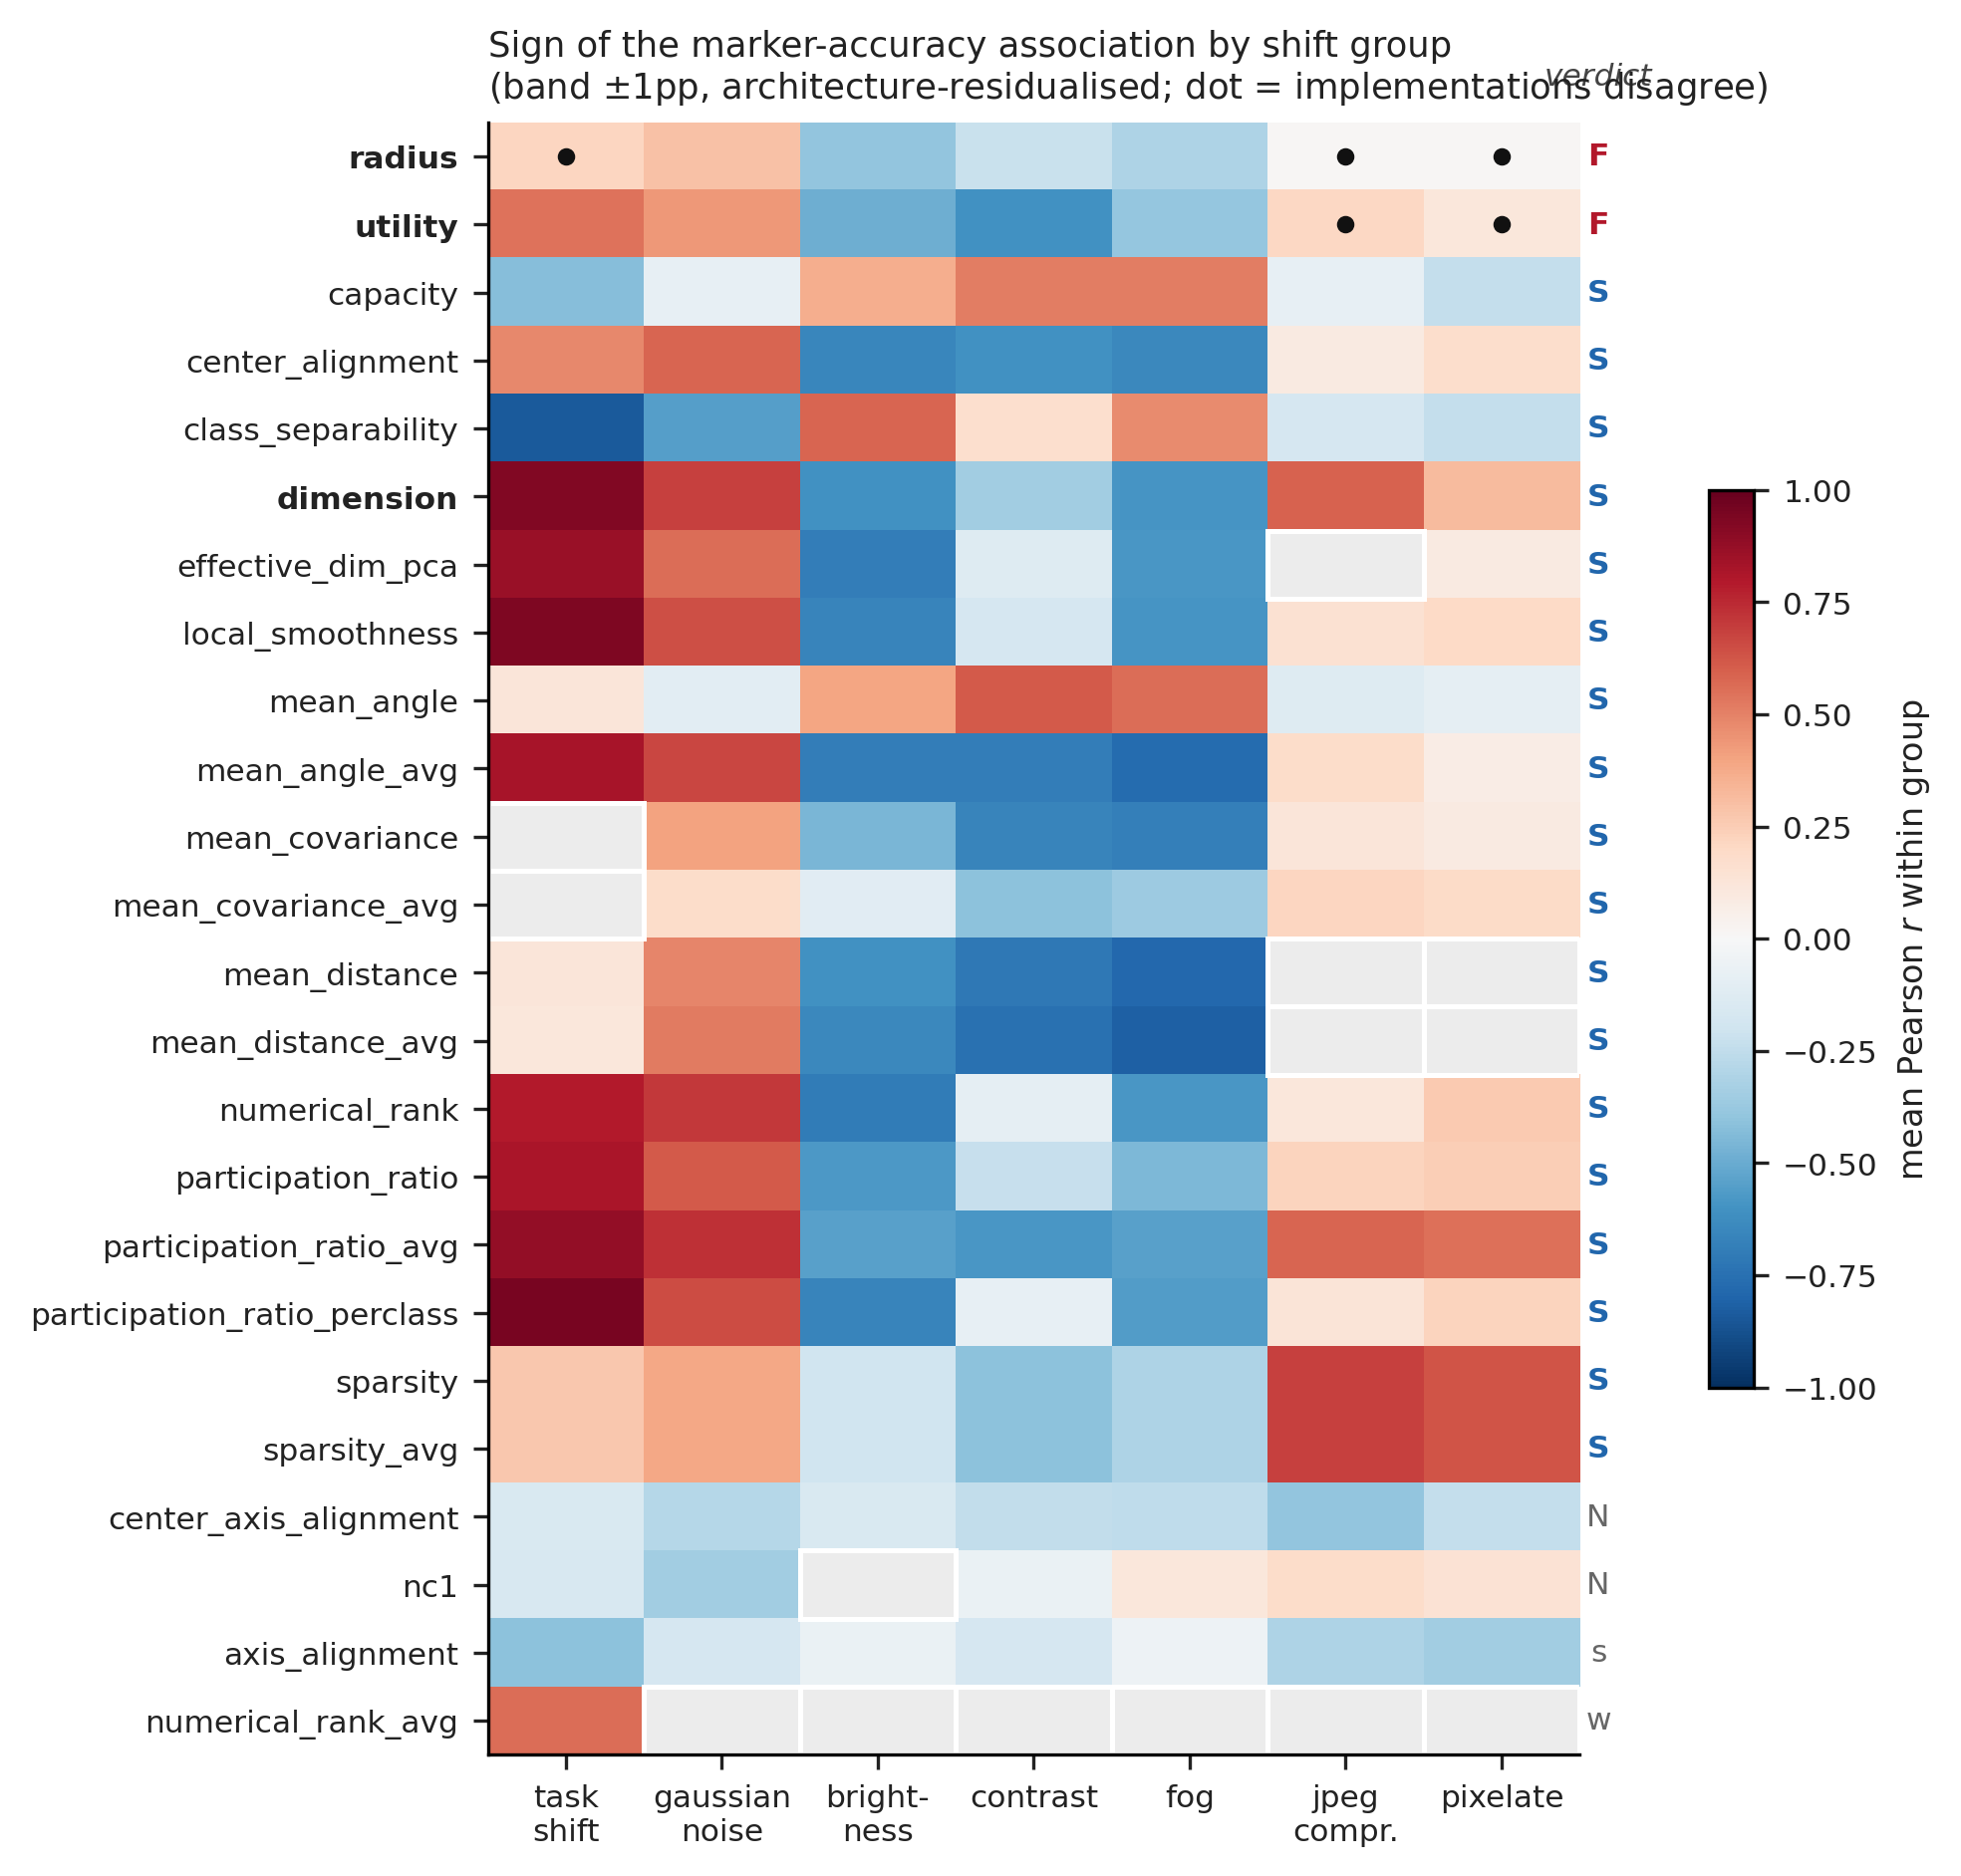
\includegraphics[width=\linewidth]{figures/fig_shiftmap.png}
\caption{The full sign-stability map. Each row is one marker family; each
column is one distribution shift. Colour is the mean Pearson $r$ within that
shift (averaged over the implementations that provide the cell); a dot marks a
shift where the two implementations disagree in sign; grey means the cell is
not measurable at this bandwidth. The right margin letter is the family's
verdict (F~=~flip, S~=~shift-dependent, N~=~unstable in sample size, w/s~=
weak/stable same-sign). Eighteen of twenty-four families are
shift-dependent: the photometric and compression columns disagree in sign
with the task and noise columns for nearly every marker.}
\label{fig:shiftmap}
\end{figure}

\begin{figure}[t]
\centering
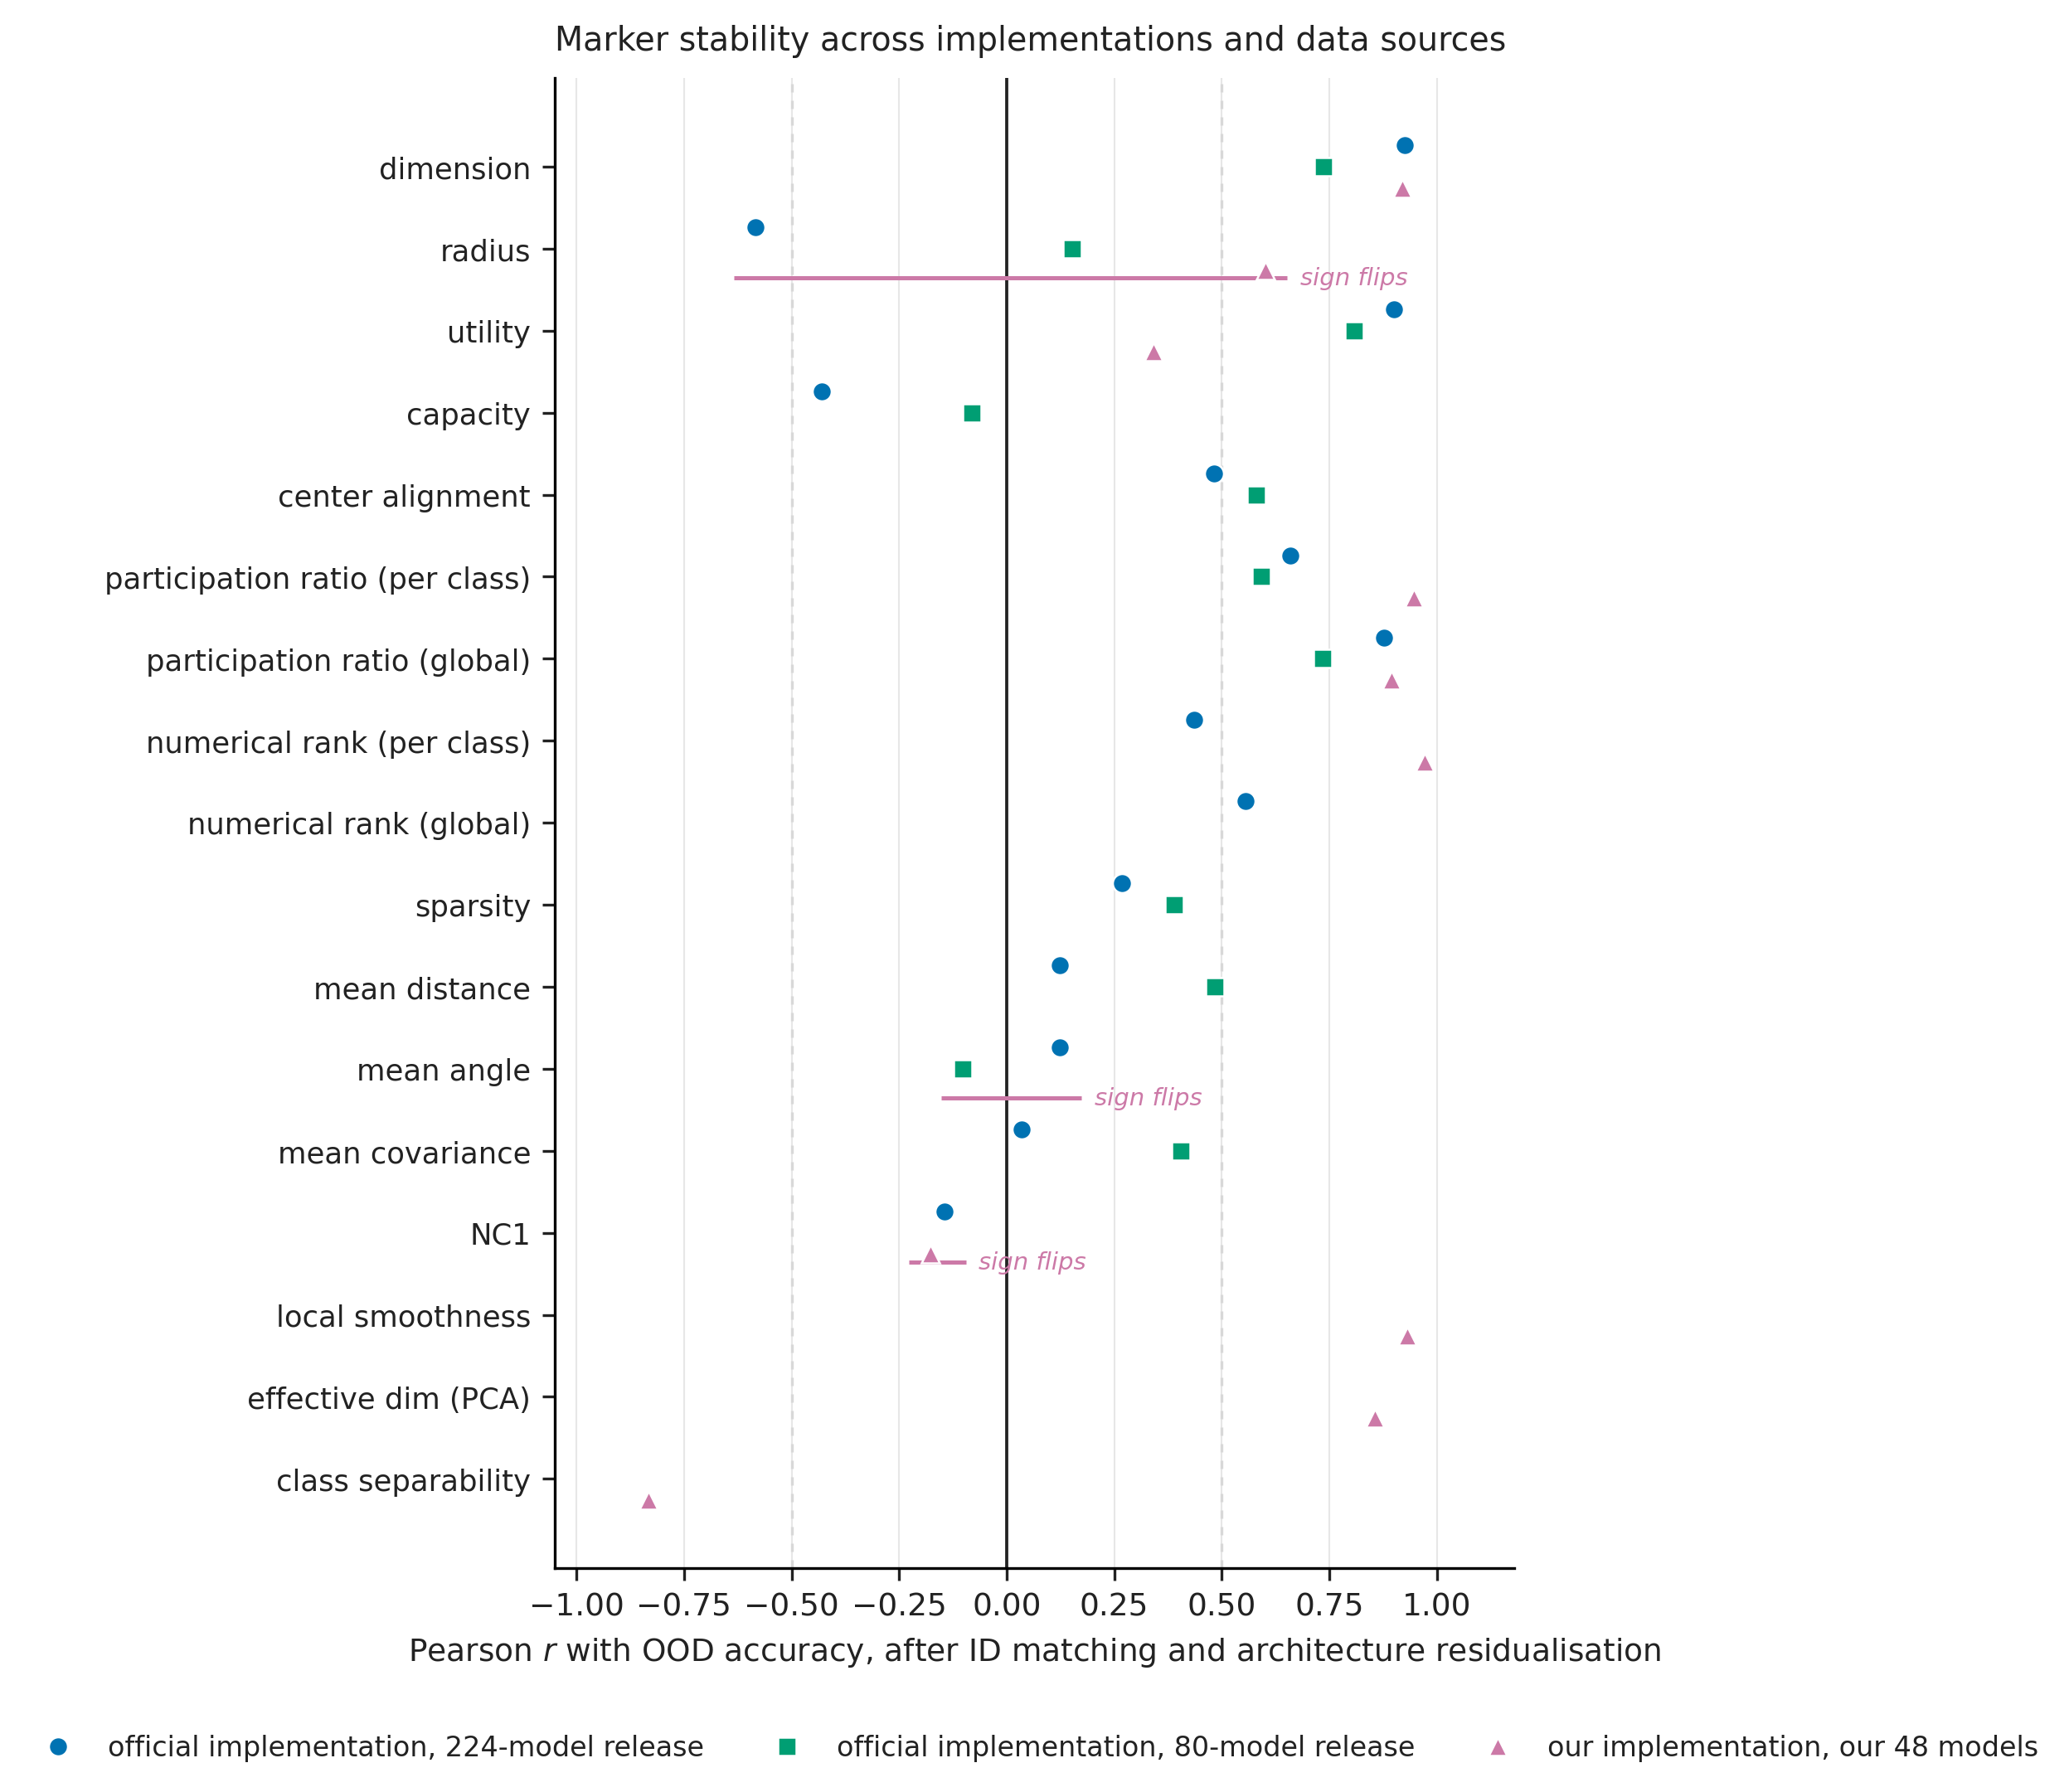
\includegraphics[width=0.85\linewidth]{figures/fig_map.png}
\caption{The implementation axis in detail: every marker measured in the
three implementation-source cells of the earlier design (reference
implementation on the two official releases; our implementation on our own
models), under the task-shift target. Each row is one marker; each symbol is
one cell; the vertical line is zero. A marker that sits on one side of zero
in one cell and the other side in another cannot be used to rank models.
This view underlies the per-family discussion below; the full
seven-shift view is Figure~\ref{fig:shiftmap}.}
\label{fig:map}
\end{figure}

\begin{table}[t]
\centering
\small
\setlength{\tabcolsep}{4pt}
\begin{tabular}{@{}llrrrrl@{}}
\hline
Family & Shift & ref.\ impl. & our impl. & $n$ (r/o) & agree & verdict \\
\hline
`dimension` & task & $+0.925$ & $+0.919$ & 106/32 & yes & \\
`dimension` & gaussian noise & $+0.737$ & $+0.623$ & 25/32 & yes & \\
`dimension` & brightness & $-0.493$ & $-0.712$ & 25/32 & yes & \\
`dimension` & fog & $-0.562$ & $-0.620$ & 25/32 & yes & \\
`dimension` & contrast & $-0.584$ & $-0.114$ & 25/32 & yes & \\
 & & & & & & shift-dep. \\
\hline
`radius` & task & $-0.584$ & $+0.602$ & 106/32 & \textbf{no} & \\
`radius` & jpeg compression & $-0.185$ & $+0.204$ & 25/32 & \textbf{no} & \\
`radius` & pixelate & $-0.283$ & $+0.301$ & 25/32 & \textbf{no} & \\
`radius` & gaussian noise & $+0.153$ & $+0.438$ & 25/32 & yes & \\
 & & & & & & flip \\
\hline
`utility` & task & $+0.901$ & $+0.342$ & 106/32 & yes & \\
`utility` & jpeg compression & $+0.542$ & $-0.133$ & 25/32 & \textbf{no} & \\
`utility` & pixelate & $+0.411$ & $-0.178$ & 25/32 & \textbf{no} & \\
`utility` & gaussian noise & $+0.808$ & $+0.061$ & 25/32 & yes & \\
 & & & & & & flip \\
\hline
`participation ratio` (global) & task & $+0.659$ & $+0.895$ & 106/32 & yes & \\
`participation ratio` (global) & brightness & $-0.532$ & $-0.622$ & 25/32 & yes & \\
`participation ratio` (global) & gaussian noise & $+0.592$ & $+0.630$ & 25/32 & yes & \\
 & & & & & & shift-dep. \\
\hline
\end{tabular}
\caption{The GLUE families and one robust generic quantity, across the shifts
that carry the argument, at a matching bandwidth of $\pm1$ pp. Pearson $r$
after ID matching and architecture residualisation; ``agree'' is sign
agreement between the two implementations within the shift; $n$ counts the
official/own models entering the cell (own-48 residualisation is
mean-centering, since the population is a single architecture). The
``verdict'' column reproduces the classification assigned by the analysis
script and stored in \texttt{results/stability\_map.json}: \emph{flip} = the
implementations disagree within a shift; \emph{shift-dependent} = one
implementation reverses sign between shifts. The full map -- twenty-four
families, seven shifts, Spearman coefficients, sample sizes, bandwidth sweep,
and the seeded half-sampling sign-retention rates -- is in
\texttt{results/stability\_map.json} and Figure~\ref{fig:shiftmap}.}
\label{tab:map}
\end{table}

\paragraph{The effective radius flips sign -- and not only between implementations.}
On the reference 224-model population the effective radius is negatively
associated with the task-shift target ($r=-0.584$, $n=106$); on our own models
it is strongly positive ($r=+0.602$, $n=32$). The middle cell is near zero
($+0.153$) and drifts negative as the band widens. This is not a bandwidth
artefact: the reference-224 correlation is negative at every bandwidth we
tested ($\pm1$ to $\pm5$ pp, from $-0.584$ to $-0.796$), while our own is
positive at every bandwidth ($+0.602$ to $+0.376$).

The full map sharpens the finding in a way the three-cell design could not:
the implementations also disagree \emph{within} a single shift. Under jpeg
compression the reference implementation gives $-0.185$ and ours $+0.204$;
under pixelation, $-0.283$ versus $+0.301$. The flip is therefore not only a
property of comparing two model populations across a task boundary -- it
appears between two implementations measuring two disjoint model sets under a
held-fixed corruption type. Where the implementations do agree on the radius
(gaussian noise: $+0.153$ and $+0.438$), both signs are positive -- but the
sign there disagrees with the task-shift cells, so the marker fails in both
directions: across implementations within a shift, and across shifts within an
implementation.

\paragraph{The effective utility flips in the compression cells.}
The utility agrees in sign between the task cells ($+0.901$ and $+0.342$) and
collapses in magnitude under our implementation. Under the compression shifts
it goes further and flips: jpeg compression $+0.542$ (reference) versus
$-0.133$ (ours), pixelation $+0.411$ versus $-0.178$. In the earlier
three-cell version of this study the utility read as ``consistent sign,
variable magnitude''; the corruption cells show that reading was an artefact
of looking at the task shift only.

\paragraph{The dimension reverses under photometric shifts -- with both implementations agreeing.}
The effective dimension is the one GLUE quantity that agrees in sign and
magnitude across implementations under the task shift ($+0.925$ on 106 models,
$+0.919$ on our 32; also $+0.737$/$+0.623$ under gaussian noise). In the
earlier version of this study we recommended it on that basis as the one
usable marker of the family. The corruption cells overturn that
recommendation. Under brightness the dimension correlates negatively with the
corrupted-test accuracy under \emph{both} implementations ($-0.493$ reference,
$-0.712$ ours; our value keeps its sign in 100\% of 1{,}000 seeded
half-samples, and the reference value is stable to the bandwidth sweep);
under fog, $-0.562$ and $-0.620$; under contrast the reference
implementation gives $-0.584$. The sign of the dimension--performance
association is a property of the shift type, not of the marker. What survives
of the earlier claim is this: the dimension is the only GLUE marker whose sign
is consistent \emph{across implementations} within every shift we measured --
but no marker, the dimension included, keeps one sign across shifts.

\paragraph{The shift axis dominates the implementation axis.}
The pattern generalises beyond the GLUE family. Eighteen of the twenty-four
families are classified shift-dependent: their sign reverses between the
task/noise cells on the one hand and the photometric/compression cells on the
other. The numerical rank is the clearest non-GLUE example ($+0.972$ on our
models under the task shift, $-0.703$ under brightness). Counting cells where
both block means are callable ($|r|\ge 0.1$), fourteen families show the
block opposition. By contrast the implementations agree with each other
far more often than not: among the twenty-one families where the task-shift
cell and the gaussian-noise cell are both callable, twenty keep the same sign
between those two cells. The dominant risk to a reported sign is not that
someone re-implements the marker; it is that someone applies it to a different
shift.

\subsection{Closing the confound: the official host protocol on our models}
\label{sec:cell4}

Every implementation-vs-population comparison so far changed two things at
once: the solver and the model set. We added a fourth cell that changes one.
We ran our solver on our forty-eight models, but embedded it in the host
protocol of the reference release: the reference feature-extraction hook
(penultimate average-pooled features), the reference per-class sampling
(fixed seed, 500 points per class), the reference downsampling, and the
reference participation-ratio and NC1 formulas. Nothing about the models
changes; nothing about the solver's numerical core changes. The cell was
registered with three criteria before it was run: ranking preservation per
marker across the two host protocols (Spearman $\rho \ge 0.95$), sign
preservation for the radius, and a reference-anchor check on the released
example model.

The signs all survive. Under the paper's protocol (ID matching at
$\pm1$\,pp, mean-centering, task-shift target, $n=32$), the dimension reads
$+0.919$ in the own-host cell and $+0.924$ in the official-host cell; the
radius $+0.602$ versus $+0.675$; the utility $+0.342$ versus $+0.507$. The
radius keeps its positive sign under the official host protocol, so the host
protocol alone does not produce the radius flip -- consistent with the flip
arising from the joint change of implementation and population, not from
either alone.

The rankings do not all survive, and the pattern of failure is informative.
The dimension's ranking is essentially invariant ($\rho = 0.963$, above the
registered $0.95$ threshold), but the radius ($\rho = 0.877$) and the
utility ($\rho = 0.804$) fall below it. The host protocol -- sampling seed,
downsampling, probe configuration -- barely disturbs a strong ranking signal
but adds substantial rank noise to weak ones (the radius and utility
correlations are $\pm 0.2$--$0.4$ to begin with). A host protocol is not a
neutral wrapper: it is one more degree of freedom in what a marker measures,
and for weak markers its perturbation is the same order as the signal.

Two further readings. First, our solver carries a constant systematic offset
against the reference values on the released example model (dimension
$+32\%$, radius $-8\%$, utility $-18\%$; across ten downsampling seeds the
spread is $\pm 4\%$, far below the offset, so it is protocol, not Monte
Carlo noise). Because the offset is constant, relative comparisons within a
cell are unaffected -- which is why the sign agreement above is meaningful
despite the offset. Second, the reference participation ratio computed in
this cell correlates with the task-shift target at $r = +0.894$ on our
models -- the same strength class as the dimension -- while the reference
NC1 does not ($r = -0.244$, Spearman $-0.062$). The strong markers are
strong under both host protocols; the weak ones are not stable under
either.

\paragraph{What this licenses.}
The practical consequence is narrower than the one we drew from the
three-cell map, and more useful. Of the three GLUE quantities that the
literature reports as interchangeable evidence of a task-relevant manifold,
none survives the combined check: the radius and the utility fail across
implementations, and the dimension fails across shifts. No marker in the map
is stable across all shifts we test. A correlation reported under one shift is
a fact about that shift, and any claim of the form ``marker $X$ predicts OOD
performance'' must name the shift in the same breath. The fourth cell
sharpens the attribution: the radius flip traces to the joint
implementation-and-population change rather than to a host protocol alone,
while the host protocol itself emerges as a further degree of freedom -- one
that leaves strong rankings untouched and perturbs weak markers at the order
of their own signal.

\section{Two reasons a marker can move}

\label{sec:degen}

\subsection{The confound and the alternative}

Suppose a marker falls and performance falls. Two readings are available.

\emph{Reading A -- the representation degraded.} The network learned a worse
representation, and the marker registers this.

\emph{Reading B -- the input carried less information.} The quantity entering
the measurement decreased, and any quantity that measures how much the
representation encodes must decrease as a consequence. This is arithmetic, not
evidence.

Reading B is not a remote possibility. It is what happens whenever the
degradation is applied to the input rather than to the training: occluding a
fraction of the image removes information, and the representation of an
information-poor input carries less information, by definition.

\begin{figure}[t]
\centering
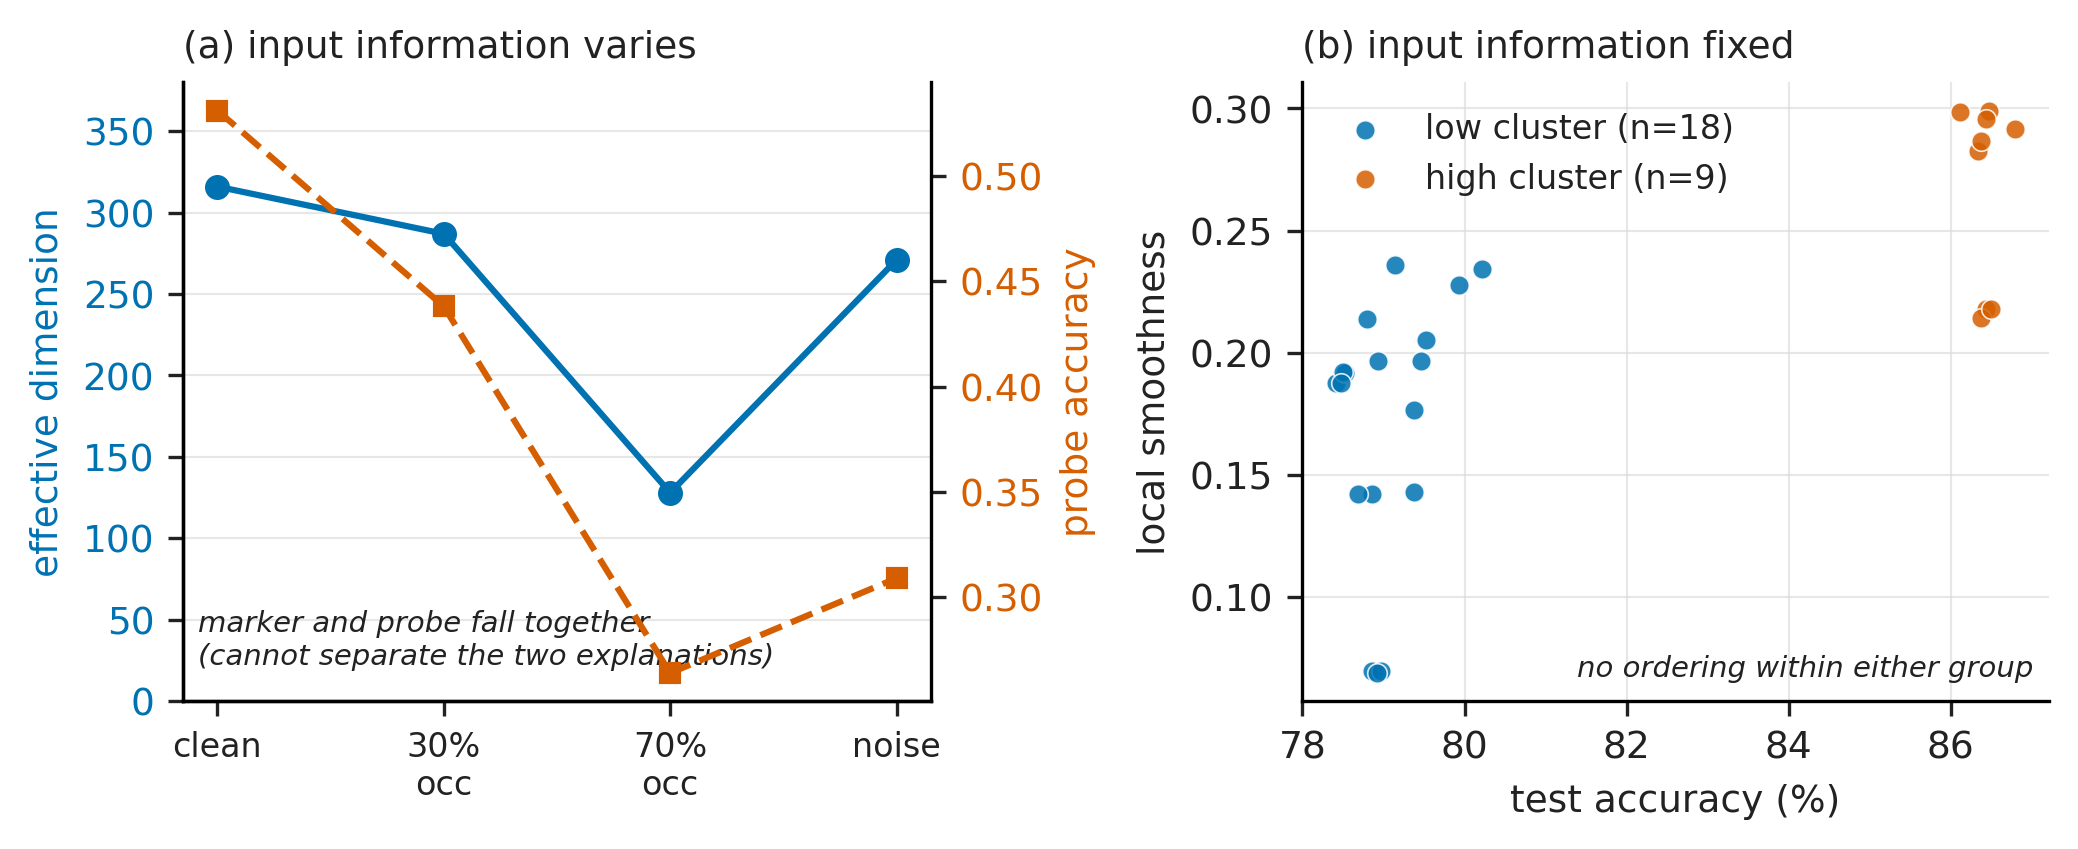
\includegraphics[width=\linewidth]{figures/fig_degeneration.png}
\caption{The two comparisons. \emph{Left}: the input information changes, and
the marker and the probe accuracy fall together -- an observation that both
readings predict. \emph{Right}: the input information is fixed and only the
training recipe varies, and the marker does not order the models within either
performance cluster.}
\label{fig:degen}
\end{figure}

\subsection{Degradation sweep: the input information changes}

We take a network trained on clean images and measure it under three degraded
inputs: 30\% and 70\% occlusion, and additive noise. Figure~\ref{fig:degen}
(left) shows the result.

\begin{table}[t]
\centering
\small
\begin{tabular}{@{}lrrr@{}}
\hline
Condition & effective dim & local smoothness & probe acc \\
\hline
clean & 316 & 0.934 & 0.531 \\
30\% occlusion & 287 & 0.910 & 0.438 \\
70\% occlusion & 128 & 0.586 & 0.264 \\
noise & 271 & 0.899 & 0.309 \\
\hline
\end{tabular}
\caption{One network under three degraded inputs. The marker falls by 59\% and
the probe accuracy by 50\% between the clean and the 70\%-occluded condition.
\textbf{Provenance:} these four rows come from a development smoke test
(ResNet-50, three seeds, averaged) rather than from the CIFAR-trained networks
used elsewhere in this paper, and the per-seed measurements behind them were not
retained; they are reported as a diagnostic illustration and are not
independently reproducible from the released artifacts. See
Limitations~\ref{sec:limitations}.}
\label{tab:degen}
\end{table}

The marker and the probe accuracy move together: the effective dimension falls
by 59\% and the probe accuracy by 50\% between the clean and the heavily
occluded condition. This is precisely what Reading B predicts, and it is also
what Reading A predicts. \textbf{The comparison cannot separate them.} A
correlational study that uses occlusion as its degradation would report a
strong, significant association and would be unable to tell whether it had
measured anything.

One detail is worth recording because it is often read as evidence for Reading
A: the marker is not equally sensitive to all degradations. It falls most
under 70\% occlusion, which removes structure, and least under noise, which
perturbs amplitude. So it responds to how the information was removed, not only
to how much. This is compatible with both readings and does not decide between
them.

\subsection{Recipe sweep: the input information is fixed}

The discriminating experiment holds the input distribution constant and varies
only the training. We trained 42 ResNet-18 networks on CIFAR-10 -- 14 recipes
crossed with 3 seeds -- where the recipes span data augmentation, label
smoothing, label noise, weight decay, learning rate, epoch budget, and
deliberate overfitting. Every network sees exactly the same clean inputs, so
the information confound is excluded by construction, and the only thing that
differs is the quality of the learned representation.

If a marker measured representational quality, it would order these recipes by
quality. It does not.

\begin{table}[t]
\centering
\small
\begin{tabular}{@{}lrrrr@{}}
\hline
Marker & pooled $r$ & $p$ & $\rho$ & within-recipe $r$ \\
\hline
`effective\_dim` & $-0.483$ & 0.0012 & $-0.536$ & $-0.443$ \\
`local\_smoothness` & $-0.452$ & 0.0027 & $-0.338$ & $-0.079$ \\
`spectral\_entropy` & $-0.410$ & 0.0070 & $-0.185$ & $-0.521$ \\
`criticality\_proxy` & $-0.217$ & 0.1678 & $-0.015$ & $+0.352$ \\
\hline
`silhouette\_gap` (trivial) & $+0.768$ & $<10^{-4}$ & $+0.732$ & --- \\
`linear\_probe\_acc` (trivial) & $+0.993$ & $<10^{-4}$ & $+0.953$ & --- \\
\hline
\end{tabular}
\caption{42 networks, 14 recipes $\times$ 3 seeds, all trained on identical
clean inputs. The two trivial markers use test labels and are a restatement of
the target. The within-recipe column removes the recipe mean from both
variables, so it asks whether the marker distinguishes networks that differ
only in their random seed.}
\label{tab:recipe}
\end{table}

\paragraph{The pooled correlation is negative and is not a gradient.}
The pooled correlation of every non-trivial marker with test accuracy is
negative (Table~\ref{tab:recipe}), the opposite of what a quality measure
would give. And the reason is visible in the distribution: test accuracy is
sharply bimodal, with networks that trained successfully and networks that
collapsed, and nothing in between. The correlation is a separation between the
two groups, not a relationship.

\paragraph{Inside a cluster there is nothing.}
Restricting to the high-performing cluster (three recipes, $n=9$), the
correlation between local smoothness and accuracy is $-0.053$ ($p=0.891$). The
effective dimension takes the same value for all nine networks, so the
correlation is undefined -- the marker does not vary at all in the region where
the representation is best, and so cannot order it. The direct comparison is
stark: the best and the second-best recipe differ in test accuracy by 0.001
and in local smoothness by 0.074. (The accuracy difference is smaller than the
seed-to-seed spread of either recipe, so it should not be read as a ranking at
all; what the comparison establishes is that the smoothness gap is two orders
of magnitude larger than the accuracy gap, not that the top two recipes are
distinguishable.)

\paragraph{The marker measures the recipe, not the network.}
Removing the recipe mean from both variables and correlating the residuals
asks whether the marker distinguishes networks that differ only in their random
seed. For local smoothness the answer is no: $r=-0.079$ ($p=0.62$). The marker's
value is essentially a property of the recipe.

\subsection{One thing the markers are good for}

The same measurements separate training failure from training success with
accuracy: the criticality proxy reaches an AUC of 0.866 at distinguishing
collapsed networks from healthy ones (permutation test over label shuffles,
20{,}000 draws, $p=0.003$; 6 failures against 36 healthy runs), the effective
dimension and local smoothness reach 0.750 ($p=0.054$ and $p=0.053$), and
spectral entropy's 0.606 is statistically indistinguishable from chance
($p=0.43$). Only the first would survive a conventional correction for
testing four markers at once, and we report the other three exactly because
of that: most geometric markers do \emph{not} separate the two regimes
reliably, which is consistent with the reading above. This is a weaker use
than grading quality, and it is a defensible one --- for the marker that
clears the bar. Detecting that a run went wrong
does not require the quantity to be a graded measure of quality; it only
requires it to differ between the two regimes. We think this is the right way
to use geometric markers today: as a health check on a training run where the
specific marker has been validated for that purpose, and not as a measure of
the representation.

\section{What to do with the next marker}

\label{sec:practice}

The two comparisons above give a procedure. A candidate geometric marker should
be asked five questions, in this order.

\begin{enumerate}
\item \textbf{Does it survive the recipe sweep?} Train several networks on
      identical inputs that differ only in the recipe, and require the marker
      to order them by quality. This is cheap -- no new architecture is needed
      -- and it is the test that disqualifies the markers studied here. A
      marker that moves with the recipe rather than with the network has not
      been shown to measure anything about the representation.
\item \textbf{Does it survive an implementation change?} Compute the marker
      with two independent implementations, or on two populations that share
      no models, and require the sign of the association to agree. This is the
      test that disqualifies the effective radius.
\item \textbf{Does it survive a change of shift?} Recompute the correlation
      with at least one target from a different shift family -- a corruption
      type if the claim was made under task shift, or the reverse -- and
      require the sign to hold. This is the test that the earlier version of
      this study did not run, and the one that disqualifies the effective
      dimension. It is also the cheapest of the three: the corruption-cell
      targets are public, and re-running a correlation costs nothing.
\item \textbf{Does it survive a change of host protocol?} Re-measure the
      same models with the same solver embedded in a different host
      protocol -- different sampling seed, downsampling rule, or probe
      configuration -- and require the ranking to hold
      (Section~\ref{sec:cell4}). This is the fourth of the five tests and
      the cheapest to run, since it needs no new models and no new shifts:
      on our data it left a strong marker's ranking intact
      ($\rho = 0.963$) while dragging two weak markers below the threshold
      we had registered ($\rho = 0.877$, $0.804$).
\item \textbf{If it is a fitted statistic, does it survive re-sampling the
      run?} When the candidate quantity is not a point measurement but a
      parameter fitted to a response curve (an exponent, a threshold, a
      half-life), estimate it under independent training randomness of the
      same configuration and require the spread across draws to be small
      relative to the effect being claimed. In the companion study cited
      in the Limitations, $15\%$ of single-curve draws were excursions
      that deviated from their per-seed cores by up to $0.47$ ---
      several times any across-seed difference measured in that batch
      --- and no two- or three-point proxy reproduced the full-curve
      ranking, so the full curve had to be re-run per draw. A shape
      statistic quoted from a single run is one draw from a
      distribution the claim has not yet characterized.
\end{enumerate}

A marker that passes all five is worth taking seriously. None of the
twenty-four families studied here does: the map is the record of that fact.
The most common failure in the current literature is not a wrong sign but an
unreported one -- a correlation measured under a single shift and read as a
property of the marker. Reporting the shift alongside the coefficient, as one
reports the dataset alongside an accuracy, would have caught every flip in
this paper at the point of writing.

None of the five tests is expensive, and all are currently skipped. We hope
that reporting them as a standard part of any claim about a geometric
predictor will make the more confident claims in the literature easier to
evaluate.

\section{Limitations}

\label{sec:limitations}

\begin{enumerate}
\item Our own GLUE implementation follows the published algorithm but does not
      reproduce two steps of the reference implementation (per-manifold-pair
      analysis and Gaussianization preprocessing). We therefore use it only
      for relative comparison within our own model family, never against
      absolute reference values. A difference between implementations could
      in principle come from our implementation rather than from the reference
      one. Two facts bound this concern without removing it: the radius
      sign also differs between the two official releases, which do not
      involve our implementation at all; and under brightness and fog the two
      implementations agree on the sign that refutes the dimension, so the
      photometric reversal is not an artefact of our solver.
\item The recipe sweep uses one architecture on one dataset. Its finding --
      that the markers track the recipe rather than the network -- is
      consistent across the three seeds and across the fourteen recipes, but
      we have not shown that it generalizes to other architectures.
\item The corruption cells of the map use corrupted-test accuracy as the
      target, not the class-level transfer probe the task cells use; the two
      targets differ in construction (Section~\ref{sec:map}). The
      shift-dependent verdicts therefore compare associations measured
      against different operationalisations of ``performance under shift''.
      We regard this as intrinsic to the question -- a shift defines its own
      target -- but a design that held the target fixed and varied only the
      inputs would separate the two effects.
\item The six corruption scenarios of the official release are correlated
      with one another (the same 80 models enter every cell), so the six
      corruption columns are not six independent replications of the
      photometric/compression pattern. The independent replication of that
      pattern comes from our own 48 models, which the official release does
      not contain.
\item We did not have access to the reference implementation of the GLUE
      solver, so the three-cell design varies the implementation and the
      population together. We cannot separate the two effects within our own
      models; a design that holds the population fixed and varies only the
      implementation would sharpen the claim, and we regard it as the most
      valuable follow-up. A fourth cell
      (Section~\ref{sec:cell4}) narrows this gap from the protocol side: it
      holds the population and the solver fixed and varies only the host
      protocol around the solver, showing that the host protocol alone does
      not reproduce the radius flip but does perturb weak-marker rankings.
      Full separation -- holding everything fixed and swapping only the
      solver's numerical core -- still requires the reference solver's
      private internals, which remain unavailable; if access is granted the
      swap becomes a direct check.
\item The degradation sweep is a single network with three seeds, reported as
      the mean. It is a diagnostic rather than an experiment: it establishes
      that the degradation sweep cannot discriminate the two readings, not
      that any particular marker fails. Two further caveats apply to
      Table~\ref{tab:degen} specifically. The network is a ResNet-50 measured
      on a non-CIFAR image set, not one of the CIFAR-trained networks used in
      the recipe sweep; and the per-seed measurements behind the reported means
      were not retained, so those four rows cannot be re-derived from anything
      in the released artifacts. We keep the table because it illustrates the
      point of the section, but a reader should treat it as an illustration
      with a stated provenance rather than as a reproducible measurement.
\item We evaluate the markers against one OOD target per cell. The full map
      multiplies the shifts but not the targets within a shift; whether the
      stability classes reported here depend on the choice of target within a
      shift family is an open question.
\item The single-sample fragility documented here for correlations has an
      exact counterpart for \emph{fitted shape statistics}. In a companion
      study (same models, same measurement chain; preregistered log
      ADR-0016 Apps.~23--35 and ADR-0017), the power-law exponent $b$
      fitted to a five-point dose--response curve of one network was
      re-estimated under independent training randomness (same base
      checkpoint, new run seed) in a symmetric five-seed $\times$
      four-draw design (20 curves): every seed has a tight core
      (per-seed medians $0.27$--$0.45$), but $15\%$ of draws are
      \emph{excursions} up to $b=0.90$, whose anatomy is localized
      --- the lowest-dose point collapses into the placebo band
      while its denominator stays normal, levering the fitted slope
      --- and whose rerun under the same seed does not reproduce,
      so they are genuine run-level random events. Retrospective
      analysis of the curves further showed that no fixed subset of
      two or three dose points reproduces the five-point exponent
      ranking (the collapses concentrate in different dose segments
      per seed), so the effect cannot be cheaply screened. Any shape
      parameter quoted from one curve of one run should therefore be
      read as one draw from a heavy-tailed sampling distribution,
      not as a property of the architecture; cross-condition
      comparisons of such statistics need the per-condition median
      over at least four draws.
\end{enumerate}

\section{Conclusion}

\label{sec:conclusion}

Geometric markers of the representation are useful, and the way to use them
well is to stop asking them to grade quality. Our results say five things.
First, a marker that falls with performance may be telling you that the input
carried less information, and the only way to find out is to hold the input
fixed and vary the training. Second, a marker's sign is not guaranteed to
survive a change of implementation: the effective radius does not, and the
failure repeats within single shifts, not only across model populations.
Third, a marker's sign is not guaranteed to survive a change of shift either:
the effective dimension -- the one marker we had previously recommended --
reverses under photometric shifts with both implementations agreeing, and
eighteen of twenty-four families in the full map change sign between the
task/noise block and the photometric/compression block. Fourth, the
implementation--population confound does not reduce to a host-protocol
effect: re-measuring our models under the reference host protocol preserves
every sign, including the radius's positive sign on our population, while
leaving weak-marker rankings perturbed at the order of their own signal
-- so the flip traces to the joint change, and the host protocol joins the
list of degrees of freedom a marker consumer must report. Fifth, the markers
are reliable health checks on a training run and unreliable measures of a
representation. A practical conclusion follows: report the shift alongside
the coefficient, as one reports the dataset alongside an accuracy; run the
five tests of Section~\ref{sec:practice} before believing any new marker;
and treat the claims in the literature that name no shift as claims about no
particular thing.

\section*{Reproducibility statement}

\label{sec:repro}

All experiments use public data (CIFAR-10/100, CIFAR-10-C, Tiny-ImageNet) and
the public releases of the original study (MIT-licensed repository). The
protocol implementation, the analysis code, the per-model measurements, and the
trained models are released at
\href{https://github.com/zhouranxi/brainai-protocol-a}{github.com/zhouranxi/brainai-protocol-a}
and archived at \href{https://doi.org/10.5281/zenodo.23728883}{doi:10.5281/zenodo.23728883}
(concept DOI \href{https://doi.org/10.5281/zenodo.23728883}{10.5281/zenodo.23728883});
the version DOI of this record is 10.5281/zenodo.23918659.

Every number reported in this paper is re-derived from the released artifacts by
the accompanying script \texttt{code/audit\_paper\_measurement.py}, which
recomputes every coefficient, sample size and p-value quoted above --
including the full sign-stability map of
Section~\ref{sec:map}, read directly from
\texttt{results/stability\_map.json} -- and checks each against the value
written here. The fourth-cell numbers of Section~\ref{sec:cell4} are read
from \texttt{results/glue\_cell4\_own48.json} (48 rows) and
\texttt{results/glue\_own48\_results.json} against the registered criteria
of \texttt{code/cell4\_verdict.py}; the systematic-offset calibration of our
solver is documented by the variant-scan scripts under
\texttt{code/glue\_*}.
It requires no GPU and no downloads. The same check runs automatically on every
push of the repository, so the reproducibility of this paper is continuously
machine-verified rather than asserted.

\subsection*{Ethics statement}

This study involves no human participants and no personally identifiable data:
all experiments use public benchmark datasets and publicly released per-model
measurements from a prior study. The work does not involve clinical, biometric,
or otherwise sensitive data, and no individual person is subject to evaluation.
We release the protocol implementation, the analysis code, and the trained model
checkpoints to permit independent verification and reuse. We are mindful that
the models we release are trained on datasets with known licensing terms, and we
distribute them subject to those same terms.

\subsection*{Use of AI tools}

Large language models were used as writing and coding assistants during
preparation of this manuscript: converting an internal draft to LaTeX,
assisting with routine refactoring of the analysis scripts, and re-deriving
every numeric claim from the released files with an independent verification
script. All scientific content --- the measurement-study framing, the
analyses, the interpretation, and every reported number --- was determined by
the authors, and each number is checkable against the released data by the
accompanying verification script. The authors take full responsibility for the
content of the publication.

% PLACEHOLDER -- DELETE THIS COMMENT AND THE COMMENTED SECTION BELOW BEFORE THE CAMERA-READY SUBMISSION.
% \section*{Acknowledgements}
% We thank the authors of the original study for releasing the per-model measurements that
% made the re-analysis possible, and for answering our methodological questions about the
% probe pipeline.

\bibliographystyle{tmlr}
\bibliography{references}

\end{document}
